%----------------------------------------------------------------------------
%----------------------------------------------------------------------------
Measurements of LIF from molecular iodine illuminated with red and green HeNe can be found in the literature and are performed in undergraduate labs. We repeat some of these experiments to verify the calibration procedures to acquire spectral data and the numerical model use to analyze these data. See Figures \ref{iodine_potato} and \ref{iodine_clean} for scans of a crudely prepared iodine cell and a scan from a commercially prepared cell.
%----------------------------------------------------------------------------
%----------------------------------------------------------------------------
%bb defines the bounding box for the pdf
%viewport defines the area of the pdf used
%in sidewaysfigure the last entry in bb moves the caption toward/away the pic
%in sidewaysfigure the second entry in bb moves the pic toward/away the caption
%----------------------------------------------------------------------------
\begin{figure}
\scalebox{0.8}[0.8]{
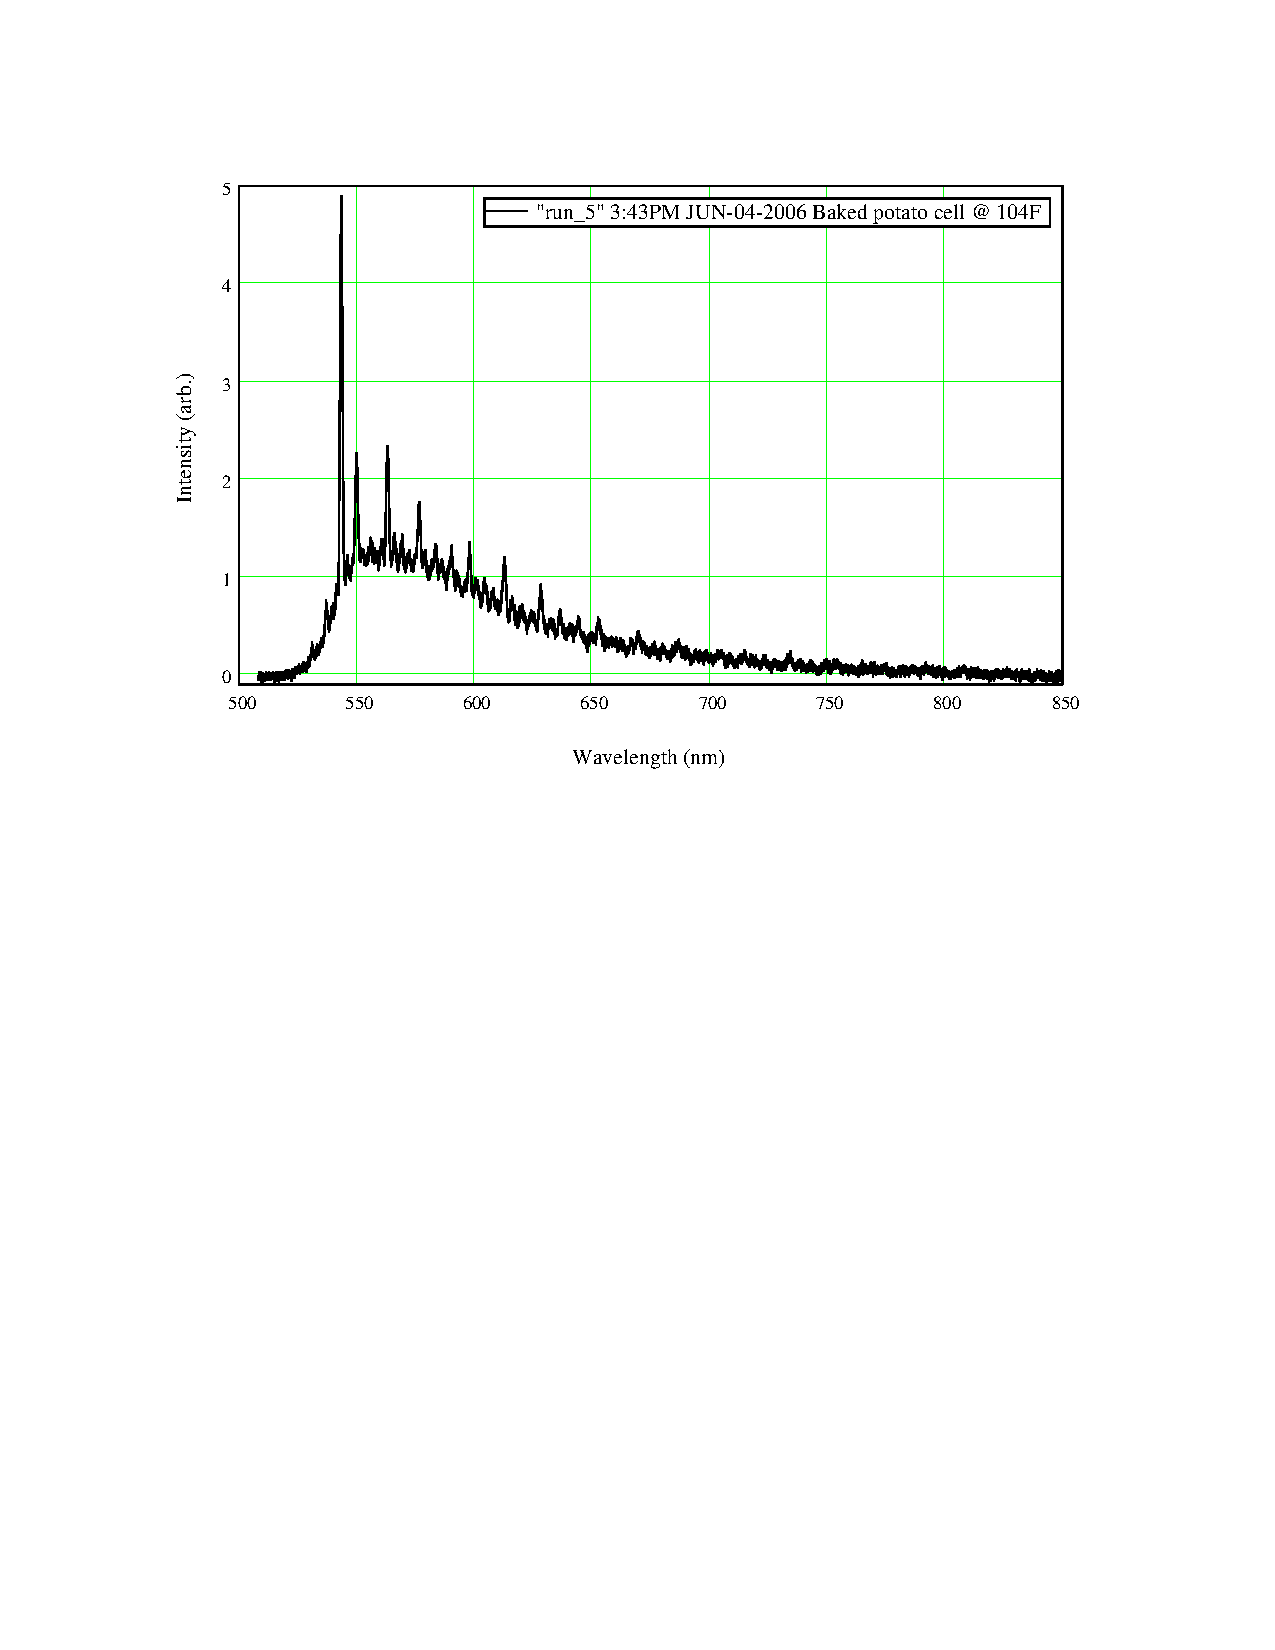
\includegraphics[bb=40 425 489 685]
{iodine_potato/iodine_potato.pdf}
}
\caption[Red HeNe LIF from the ``baked potato'' iodine cell]{Red HeNe LIF from the ``baked potato'' iodine cell. Notice the broad pedestal absent in the ``clean'' cell scan in Figure \ref{iodine_clean} -- see Section \ref{res LIF section} for discussion.}
\label{iodine_potato}
\end{figure}
%----------------------------------------------------------------------------

%----------------------------------------------------------------------------
%bb defines the bounding box for the pdf
%viewport defines the area of the pdf used
%in sidewaysfigure the last entry in bb moves the caption toward/away the pic
%in sidewaysfigure the second entry in bb moves the pic toward/away the caption
%----------------------------------------------------------------------------
\begin{figure}
\scalebox{0.8}[0.8]{
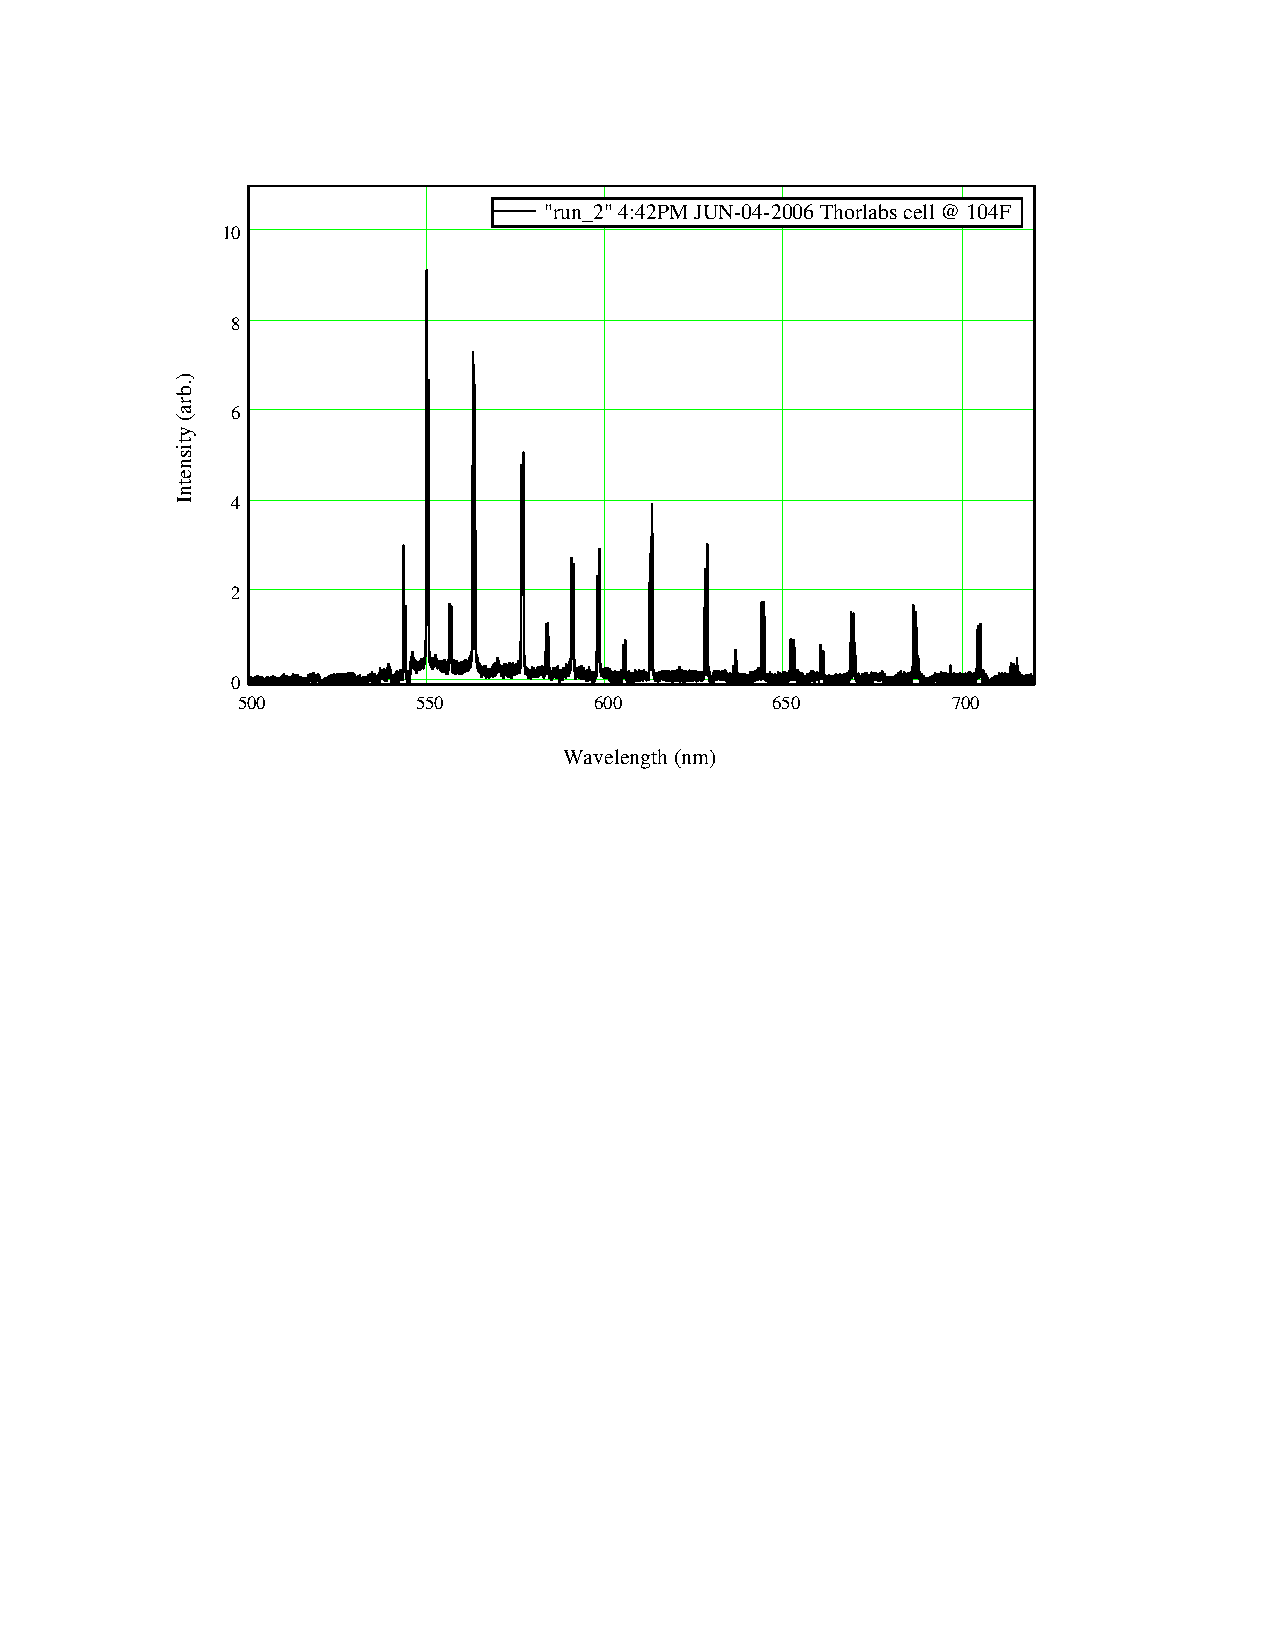
\includegraphics[bb=40 425 489 685]
{iodine_clean/iodine_clean.pdf}
}
\caption{Red HeNe LIF from a ``clean'' commercial iodine cell (Thorlabs)}
\label{iodine_clean}
\end{figure}
%----------------------------------------------------------------------------

%----------------------------------------------------------------------------

The high voltage fast rise time relay mentioned in Section \ref{Hg pulser and fast PD section} will be used to provide the fast voltage pulse that will drive the Pockels cell in the final dye laser system. The simple beam line used for the LIF measurement mentioned above is exploited to test a recently acquired Pockels cell (Cleveland Crystals Inc., Impact 8 KD*P Pockels Cell with a 532 nm AR coating). A crude Pockels cell mount is quickly constructed and the red HeNe output is sent through two crossed polarizers with the Pockels cell mounted in between. Alignment proved difficult (this knowledge prompted the design and construction of a new Pockels cell mount); however, once setup properly, the Pockels cell/Hg pulser system worked well (see Sections \ref{DC test section} and \ref{Pockels cell pulse section} or UH notebook UH--015 page 59). 
%----------------------------------------------------------------------------
%----------------------------------------------------------------------------
